\chapter{结论与展望}\label{chap:conclusion-outlook}

本文围绕 Unix V6++ 教学操作系统面向 RISC-V 平台的移植与 Rust 重构展开研究。在保持 Unix V6++ 原有教学语义和用户态使用方式的基础上，系统将重构前 \verb|main| 分支中面向 IA-32/C++/PC 设备模型的内核，迁移为面向 RISC-V/QEMU virt 平台的 Rust 内核，并完成启动、地址空间、中断异常、系统调用、进程管理、设备适配、Shell 交互和构建验证等工作。本章总结全文工作，分析其实践价值，并说明当前系统仍可继续完善的方向。

\section{工作总结}

本文分析了原 Unix V6++ 系统的结构特点。重构前系统采用 C++ 语言组织内核模块，运行于 IA-32 传统 PC 平台，依赖引导扇区、保护模式、IDT、8259A、ATA/IDE 等机制完成启动、中断和设备访问。该版本为操作系统教学提供了完整而直观的 Unix V6 风格内核，但其体系结构相关代码与 x86 平台结合较紧。基于这一判断，本文的总体设计确定了以 RISC-V 平台机制为底层基础、以 Rust 内核模块为实现主体、以 Unix V6++ 教学语义为上层目标的重构路线。

平台迁移完成了 RISC-V 裸机内核的启动流程设计。系统通过 QEMU/OpenSBI 进入位于 \verb|0x80200000| 的内核入口，完成早期栈设置、BSS 清零、串口输出、链接脚本适配和初始化顺序组织；随后基于 Sv39 分页机制建立内核高地址映射、用户地址空间映射和 MMIO 设备映射，并通过 \verb|satp| 与 \verb|sfence.vma| 启用地址空间保护。物理内存管理保留内核页和用户页划分思想，接入 Buddy 分配器、slab 分配器和 Rust 全局分配器，为内核对象、用户进程图像和内核栈分配提供基础。

内核事件处理部分基于 RISC-V 特权架构重写了 Trap 框架。系统使用 \verb|stvec| 建立统一入口，通过汇编保存寄存器和关键控制状态，再由 Rust 层根据 \verb|scause| 分发系统调用、时钟中断、外部中断和异常。系统调用接口从原 x86 寄存器约定迁移到 RISC-V \verb|a0| 至 \verb|a7| 的参数传递方式，用户态 C 库通过 \verb|ecall| 进入内核，内核保留 Unix V6++ 的主要系统调用编号和语义。时钟中断、PLIC 外部中断和 UART 输入路径的接入，也使调度、TTY 和信号处理能够面向新平台协同工作。

进程管理和用户程序支持实现了进程控制块、进程状态机、优先级调度、睡眠唤醒、上下文切换以及 \verb|fork|、\verb|exec|、\verb|exit|、\verb|wait| 等核心进程系统调用。与 \verb|main| 分支中固定进程数组、x86 上下文和 PE 用户程序格式不同，当前系统使用 RISC-V \verb|TrapContext| 与 \verb|TaskContext| 表达用户态返回和内核态切换，使用 ELF64/RISC-V 作为主要用户程序格式，并由 \verb|exec| 完成程序段加载、用户栈构造和 argc/argv 传递。信号机制也被迁移到 RISC-V 上下文模型下，能够支持终端控制字符、用户发送信号和部分用户态异常到信号的转换。

设备与交互环境迁移将系统从原 PC 设备模型迁移到 QEMU virt 平台。块设备由 ATA/IDE 路径改为 VirtIO Block，外部中断由 PLIC 管理，终端输入输出由 UART、Console 字符设备和 TTY 层共同完成。文件系统和缓冲区管理作为用户态运行环境的一部分，继续提供 Unix V6 风格的文件、目录、打开文件表和文件描述符语义；Shell 和常用用户程序仍以 C 语言编写，通过 RISC-V 交叉工具链生成 ELF64 可执行文件。最终，系统能够通过 QEMU 启动到可交互 Shell，并通过 \verb|ls|、\verb|cat|、\verb|echo|、\verb|cp|、\verb|rm|、\verb|mkdir|、管道、重定向、进程和信号测试等方式验证主要功能路径。

\begin{figure}[htbp]
  \centering
  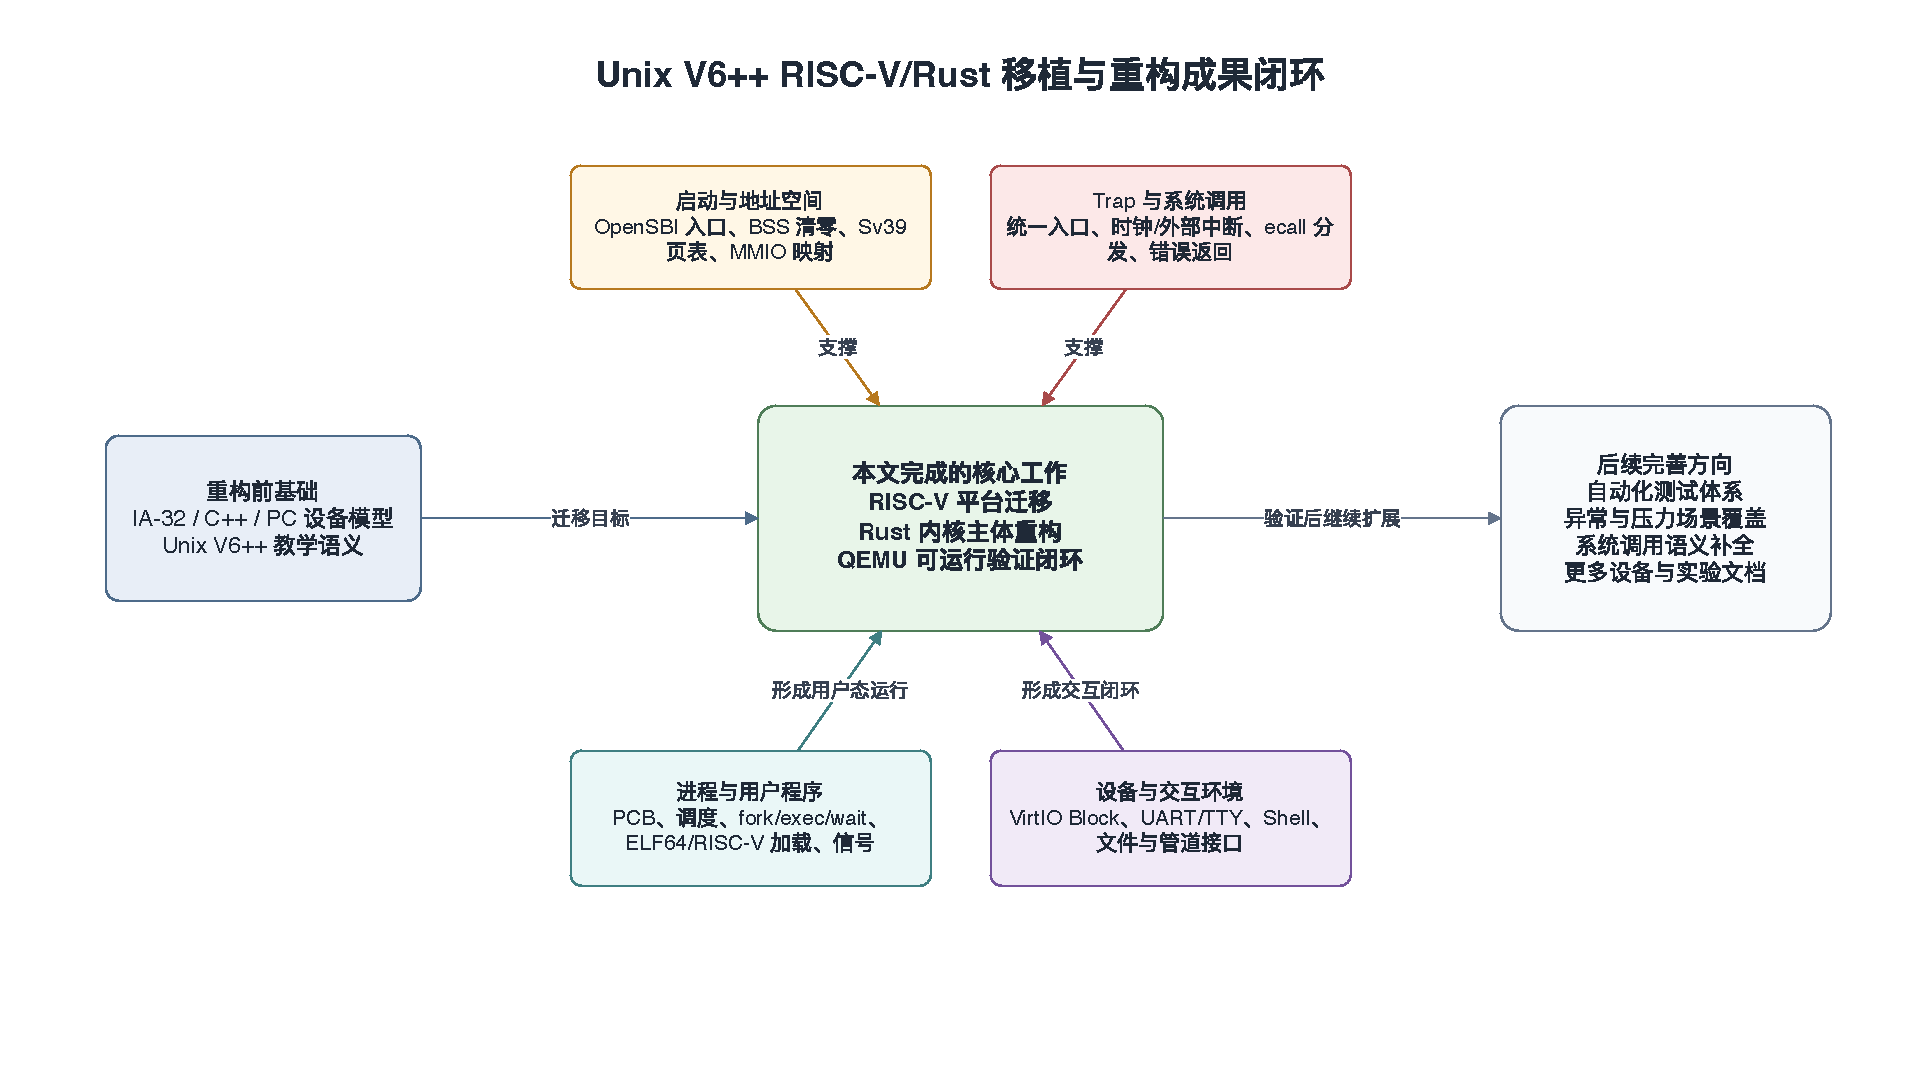
\includegraphics[width=0.95\textwidth]{figures/conclusion-roadmap.pdf}
  \caption{本文工作成果与后续完善方向}\label{fig:conclusion-roadmap}
\end{figure}

\figref{fig:conclusion-roadmap} 概括了本文工作的整体关系。重构前系统提供了 Unix V6++ 的教学基础，本文围绕 RISC-V/Rust 内核完成启动、Trap、进程、设备和交互环境的迁移，并通过构建与功能测试形成从底层初始化到用户态 Shell 的可运行闭环。与原 \verb|main| 分支相比，当前系统的变化不只是目标架构和实现语言的替换，还包括用户程序 ABI、设备访问路径、构建链和调试方式的调整。

\section{创新点与实践价值}

本文完成了 Unix V6++ 教学系统向 RISC-V 平台的系统性迁移。RISC-V 特权架构提供了异常、中断、页表和特权级接口\cite{riscv_privileged_20211203}，QEMU virt 平台则提供 OpenSBI、UART、PLIC 和 VirtIO 运行环境\cite{qemu_riscv_doc}。将 Unix V6++ 移植到这一平台后，学生可以在同一个教学系统中观察 RISC-V 启动、页表、Trap、系统调用和设备访问的完整链路，从而把操作系统原理与开放指令集架构结合起来理解。

Rust 重构重新表达了教学内核中的资源管理边界。当前系统仍然保留裸机内核不可避免的底层操作，例如页表项修改、MMIO 访问、用户指针读取和汇编上下文切换；但在这些必要的 \verb|unsafe| 边界之外，页资源、内核栈、文本段引用、inode 引用、文件引用和中断开关保护等对象更多通过所有权、生命周期、\verb|Drop| 和 RAII 风格封装表达。原 C++ 版本中不少资源释放依赖调用路径上的显式配对操作，当前 Rust 版本则把部分释放责任收束到类型本身，使读者在追踪进程退出、文件关闭和页回收时更容易看到资源由谁持有、何时释放。

Unix V6++ 的教学可识别性在重构后得到保留。本文没有把系统改造成全新的接口模型，而是继续保留 Unix V6 风格的进程状态、\verb|sleep|/\verb|wakeup|、\verb|fork|/\verb|exec|/\verb|wait|、inode、文件描述符、TTY、Shell 和常用命令。重构后系统既能展示 RISC-V/Rust 平台下的实现方式，也能让原有课程中的 Unix 风格概念继续发挥作用。学生可以先从熟悉的 Shell 命令和系统调用现象进入，再逐步追踪到 RISC-V Trap、页表和设备驱动层。

当前仓库形成了可重复的构建与验证流程。Makefile 统一组织 Rust 内核、C 用户库、Shell、用户程序、文件系统镜像和 QEMU 启动目标，能够生成 \verb|src/kernel.elf| 与 \verb|target/disk.img|，并通过 \verb|qemu-system-riscv64| 的 virt 机器运行。相较于只完成内核局部模块迁移，这种从内核到用户态、从构建到运行的闭环更适合毕业设计成果展示，也便于后续课程实验继续扩充测试和功能。

\section{不足与后续工作}

当前系统已经具备教学内核所需的基本运行闭环，但仍存在一些可以继续完善的问题。测试体系仍以构建检查、启动日志观察和 QEMU 中的交互式功能测试为主，自动化程度有限。后续可以围绕系统调用、进程生命周期、文件描述符、管道、信号和异常处理建立更系统的用户态测试集，并把测试程序纳入镜像生成和 QEMU 自动运行流程，使每次修改都能得到更明确的回归反馈。

部分 Unix 语义仍有简化空间。当前系统保留了主要系统调用和 Shell 所需接口，但部分系统调用仍为空实现或返回 \verb|ENOSYS|；\verb|wait| 对子进程退出状态和时间统计的处理也较简化；信号机制能够支持基本递送和用户处理函数，但尚未覆盖更完整的屏蔽、排队和默认动作细节。后续可以在不破坏教学内核规模的前提下，逐步补齐这些接口，使用户态程序的行为更加接近 Unix 传统语义。

异常场景和压力场景覆盖还不充分。当前功能测试主要证明系统可以启动、执行 Shell 命令、创建进程、访问文件和处理信号；对于内存不足、文件系统异常、设备 I/O 错误、频繁创建退出进程、深层管道组合和非法用户指针等情况，还需要更细致的验证。内核中仍保留若干必要的底层 \verb|unsafe| 操作，后续可以通过边界检查、错误路径测试和调试断言进一步缩小潜在问题范围。

作为教学操作系统，系统还可以继续完善实验材料和文档。当前论文已经沿总体设计、启动内存、中断系统调用、进程用户程序、设备交互和测试验证等线索梳理了实现路径；后续若用于课程实验，可以进一步提炼为若干可独立完成的实验任务，例如 Trap 路径跟踪、系统调用添加、用户程序加载分析、调度策略观察、TTY 控制字符处理和 VirtIO 块设备读写跟踪等。这样可以把毕业设计中的工程成果转化为更容易复用的教学资源。

本文完成了 Unix V6++ 从 IA-32/C++/PC 设备模型到 RISC-V/Rust/QEMU virt 平台的主要迁移与重构工作，保留了原教学系统的 Unix 风格语义和用户态交互方式，并形成了可构建、可运行、可测试的教学操作系统框架。当前系统还不是一个功能完备的通用操作系统，但已经能够作为理解 RISC-V 操作系统机制、Rust 内核资源管理和 Unix V6++ 教学语义迁移的实践载体。后续工作可以继续推进自动化测试、系统调用完整性、异常场景验证和教学实验化，使该系统更适合长期维护和课程使用。
